\documentclass[a4paper,oneside,14pt]{extreport}

\usepackage[T2A]{fontenc}
\usepackage[utf8]{inputenc}
\usepackage[english,russian]{babel}

%\usepackage[left=30mm, right=20mm, top=20mm, bottom=20mm]{geometry}
\usepackage[left=20mm, right=10mm, top=5mm, bottom=20mm]{geometry}

\usepackage{microtype}
\sloppy

\usepackage{setspace}
\onehalfspacing

\usepackage{indentfirst}
\setlength{\parindent}{12.5mm}

\usepackage{titlesec}
\titleformat{\chapter}{\LARGE\bfseries}{\thechapter}{14pt}{\LARGE\bfseries}
\titlespacing*{\chapter}{\parindent}{0mm}{5mm}
\titleformat{\section}{\Large\bfseries}{\thesection}{14pt}{\Large\bfseries}

\addto{\captionsrussian}{\renewcommand*{\contentsname}{Содержание}}
\usepackage{natbib}
\renewcommand{\bibsection}{\chapter*{Список использованных источников}}

\usepackage{caption}

\usepackage{wrapfig}
\usepackage{float}

\usepackage{graphicx}
\newcommand{\imgwc}[4]
{
	\begin{figure}[#1]
		\center{\includegraphics[width=#2]{inc/img/#3}}
		\caption{#4}
		\label{img:#3}
	\end{figure}
}
\newcommand{\imghc}[4]
{
	\begin{figure}[#1]
		\center{\includegraphics[height=#2]{inc/img/#3}}
		\caption{#4}
		\label{img:#3}
	\end{figure}
}
\newcommand{\imgsc}[4]
{
	\begin{figure}[#1]
		\center{\includegraphics[scale=#2]{inc/img/#3}}
		\caption{#4}
		\label{img:#3}
	\end{figure}
}

\usepackage{pgfplots}
\pgfplotsset{compat=newest}

\usepackage{listings}
\usepackage{listingsutf8}
\lstset{
	basicstyle=\footnotesize\ttfamily,
	keywordstyle=\color{blue},
	stringstyle=\color{red},
	commentstyle=\color{gray},
	numbers=left,
	numberstyle=\tiny,
	numbersep=5pt,
	frame=false,
	breaklines=true,
	breakatwhitespace=true,
	inputencoding=utf8/koi8-r
}

\lstdefinestyle{c}{
	language=C++,
	backgroundcolor=\color{white},
	basicstyle=\footnotesize\ttfamily,
	keywordstyle=\color{blue},
	stringstyle=\color{red},
	commentstyle=\color{gray},
	directivestyle=\color{orange},
	numbers=left,
	numberstyle=\tiny,
	stepnumber=1,
	numbersep=5pt,
	frame=single,
	tabsize=4,
	captionpos=t,
	breaklines=true,
	breakatwhitespace=true,
	escapeinside={\#*}{*)},
	morecomment=[l][\color{magenta}]{\#},
	columns=fullflexible
}

\newcommand{\code}[1]{\texttt{#1}}

\usepackage{amsmath}
\usepackage{amssymb}

\usepackage[unicode]{hyperref}
\hypersetup{hidelinks}

\makeatletter
\newcommand{\vhrulefill}[1]
{
	\leavevmode\leaders\hrule\@height#1\hfill \kern\z@
}
\makeatother

\begin{document}

\begin{titlepage}
	\centering
	
	\vspace{-2.2mm}
	\vhrulefill{0.9mm}\\
	\vspace{-7mm}
	\vhrulefill{0.2mm}\\
	\vspace{2mm}
	
	\vspace{50mm}
	
	\vspace{30mm}
	
	\textbf{Отчет по лабораторной работе №7}\\
	По курсу: <<Фильтрация и прогнозирование данных>>\\
	Тема: <<Решение обратной задачи>>\\
	
	\vspace{60mm}
	
	\hspace{70mm} Студент:       \hfill Пронин~А.~С.\\
	\hspace{70mm} Группа:        \hfill МСМТ231\\
	\hspace{70mm} Преподаватель: \hfill Зотов~Л.~В.\\
	%	\hspace{70mm} Оценка:        \hfill \hrulefill\\
	
	\vfill
	
	Москва\\
	\the\year
\end{titlepage}

\setcounter{page}{2}

\chapter*{Лабораторная работа 4}

Задание 1 – Выполнить ССА предложенного и своего сигналов.

Предложенный сигнал представляет собой сумму двух гармоник (рис. \ref{task1_garm1}):

\begin{figure}[!h]
	\center{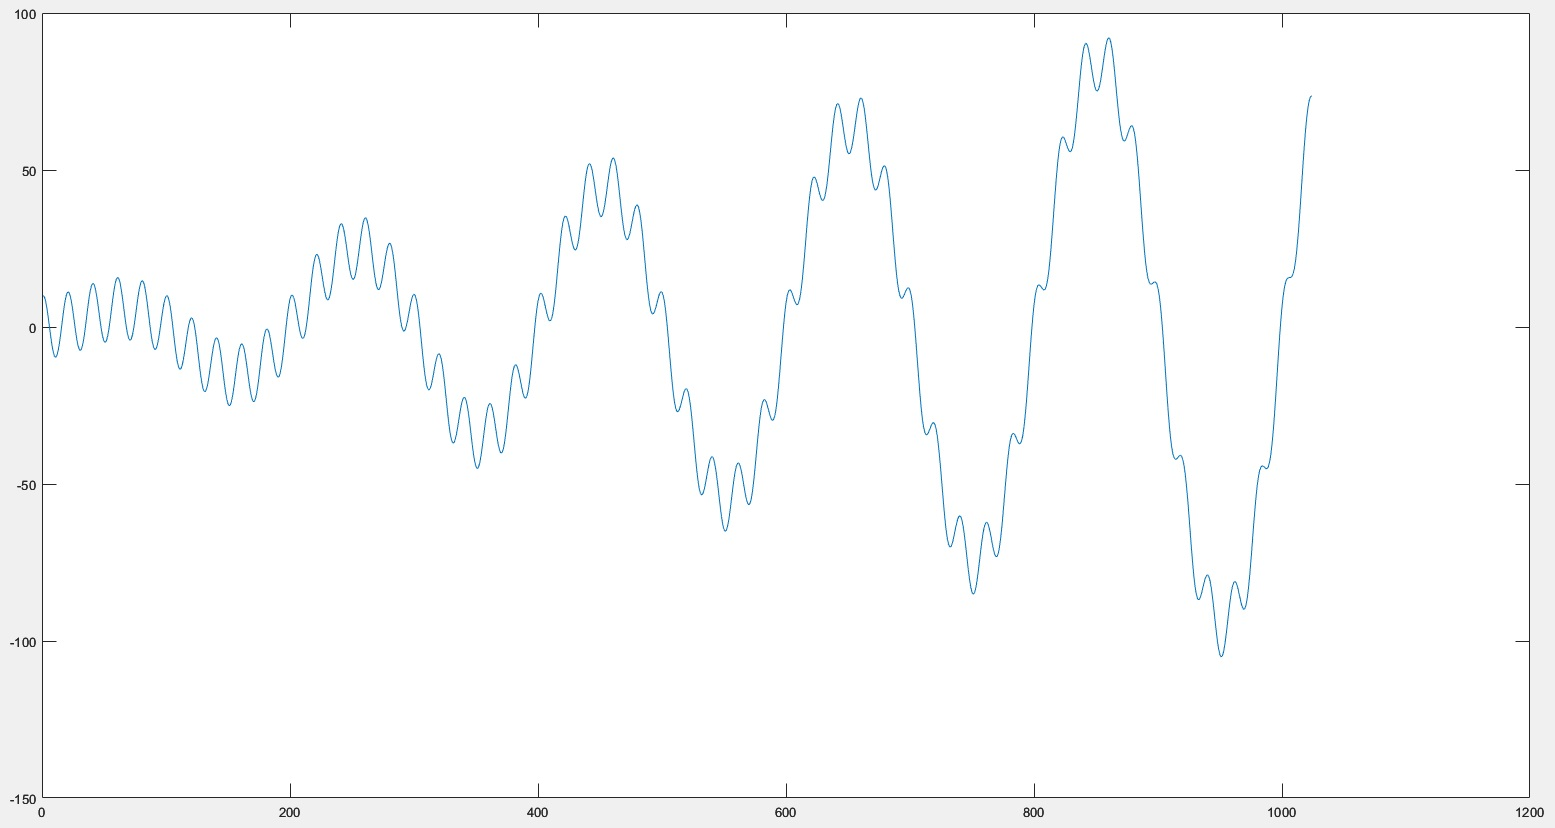
\includegraphics[width=0.9\linewidth]{inc/task1_garm1}}
	\caption{Сигнал из примера}
	\label{task1_garm1}
\end{figure}

На рисунке \ref{task1_signal1} представлены составляющие сигнала и тренд:

\begin{figure}[!h]
	\center{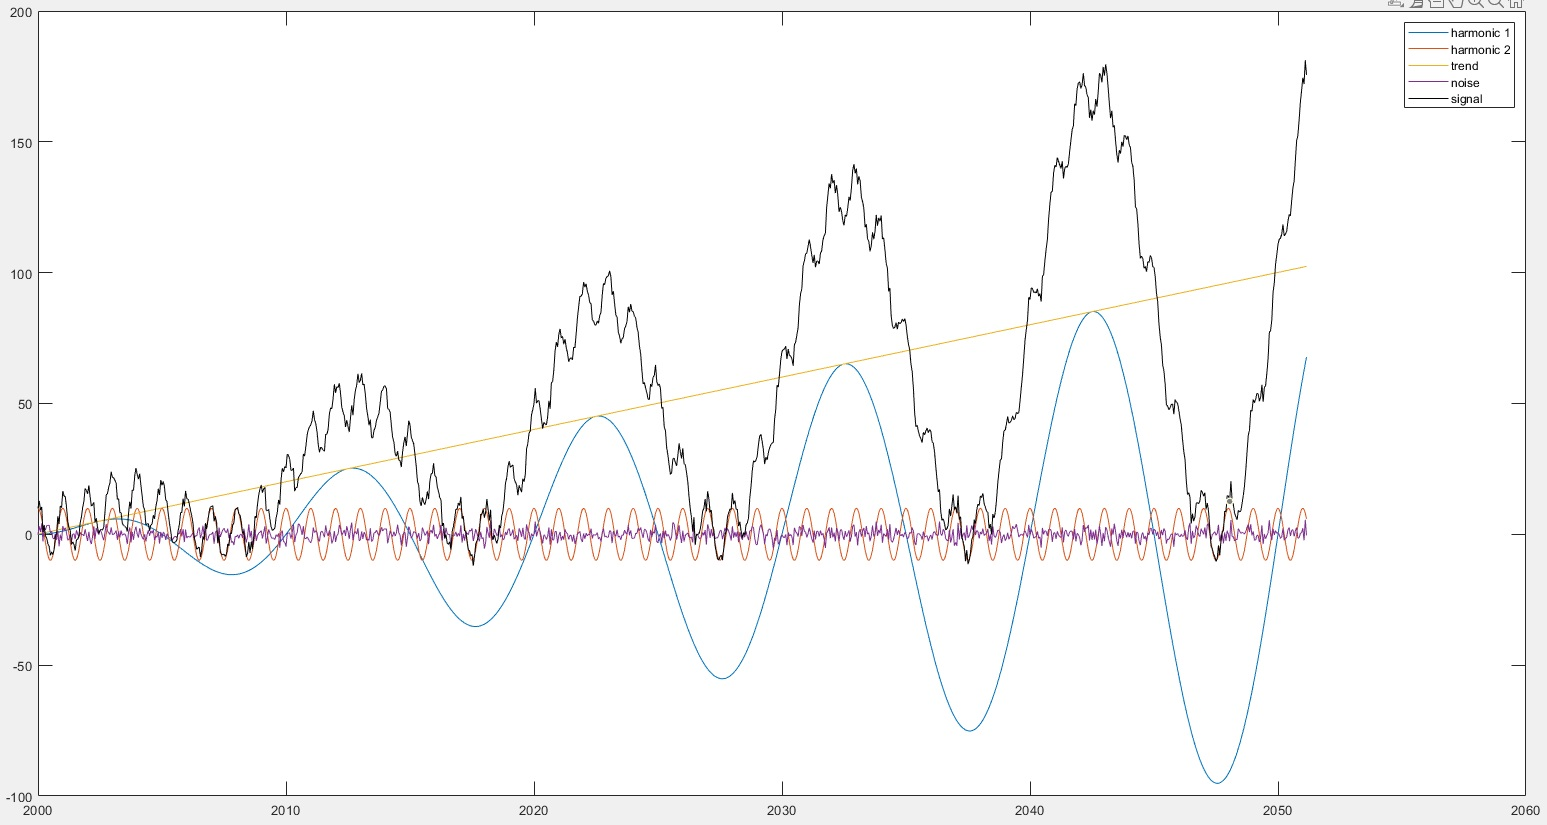
\includegraphics[width=1\linewidth]{inc/task1_signal1}}
	\caption{Сигнал с шумом и его составляющие}
	\label{task1_signal1}
\end{figure}

\newpage
На рисунке \ref{task1_fft1} представлен Фурье анализ сигнала:

\begin{figure}[!h]
	\center{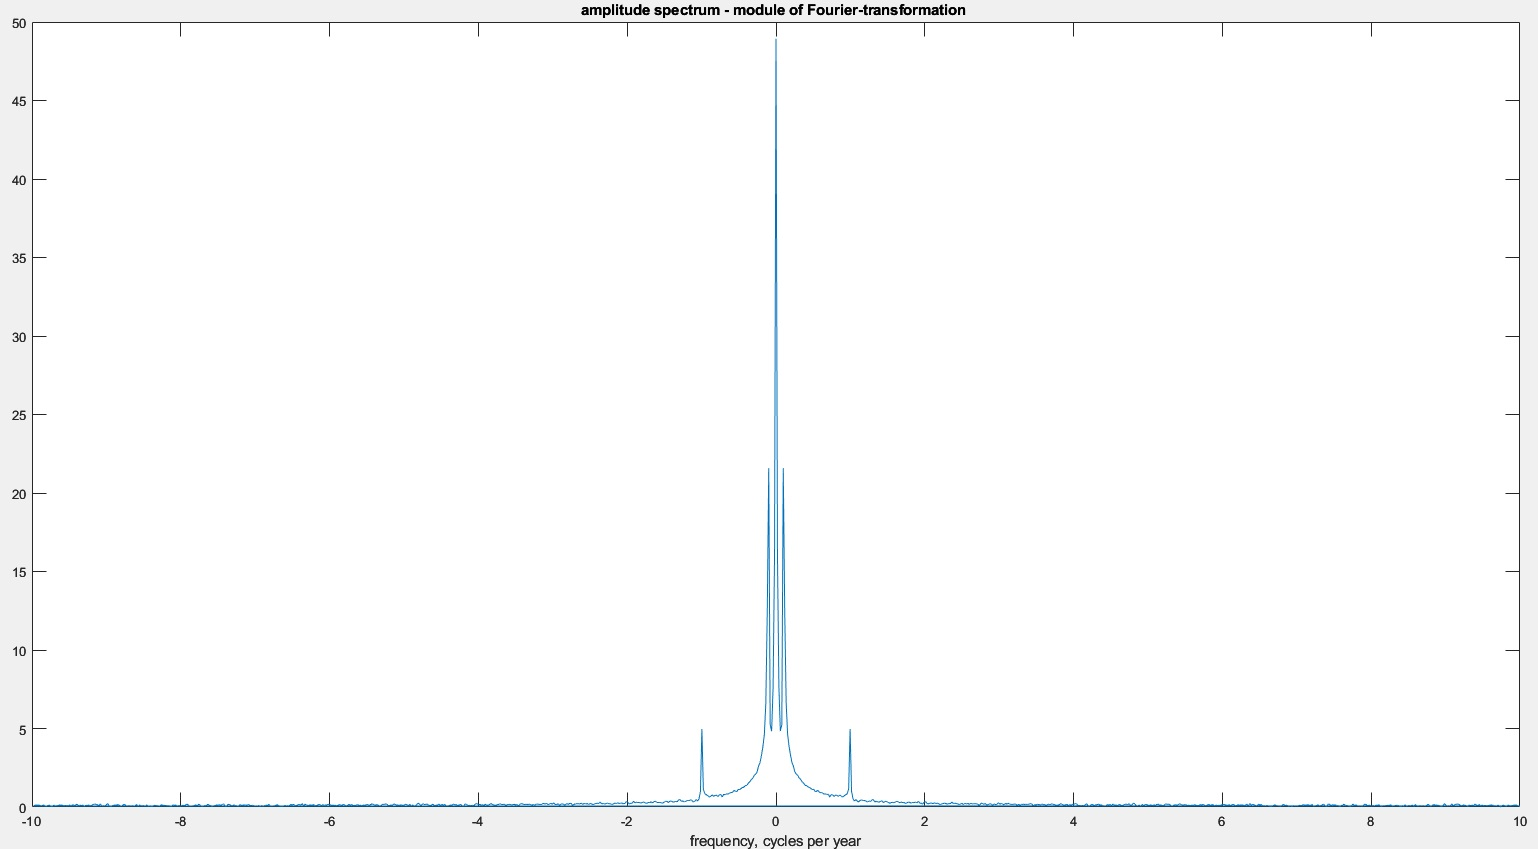
\includegraphics[width=1\linewidth]{inc/task1_fft1}}
	\caption{Фурье анализ сигнала из примера}
	\label{task1_fft1}
\end{figure}

На рисунке \ref{task1_vevlet1} представлен Вейвлет анализ сигнала:

\begin{figure}[!h]
	\center{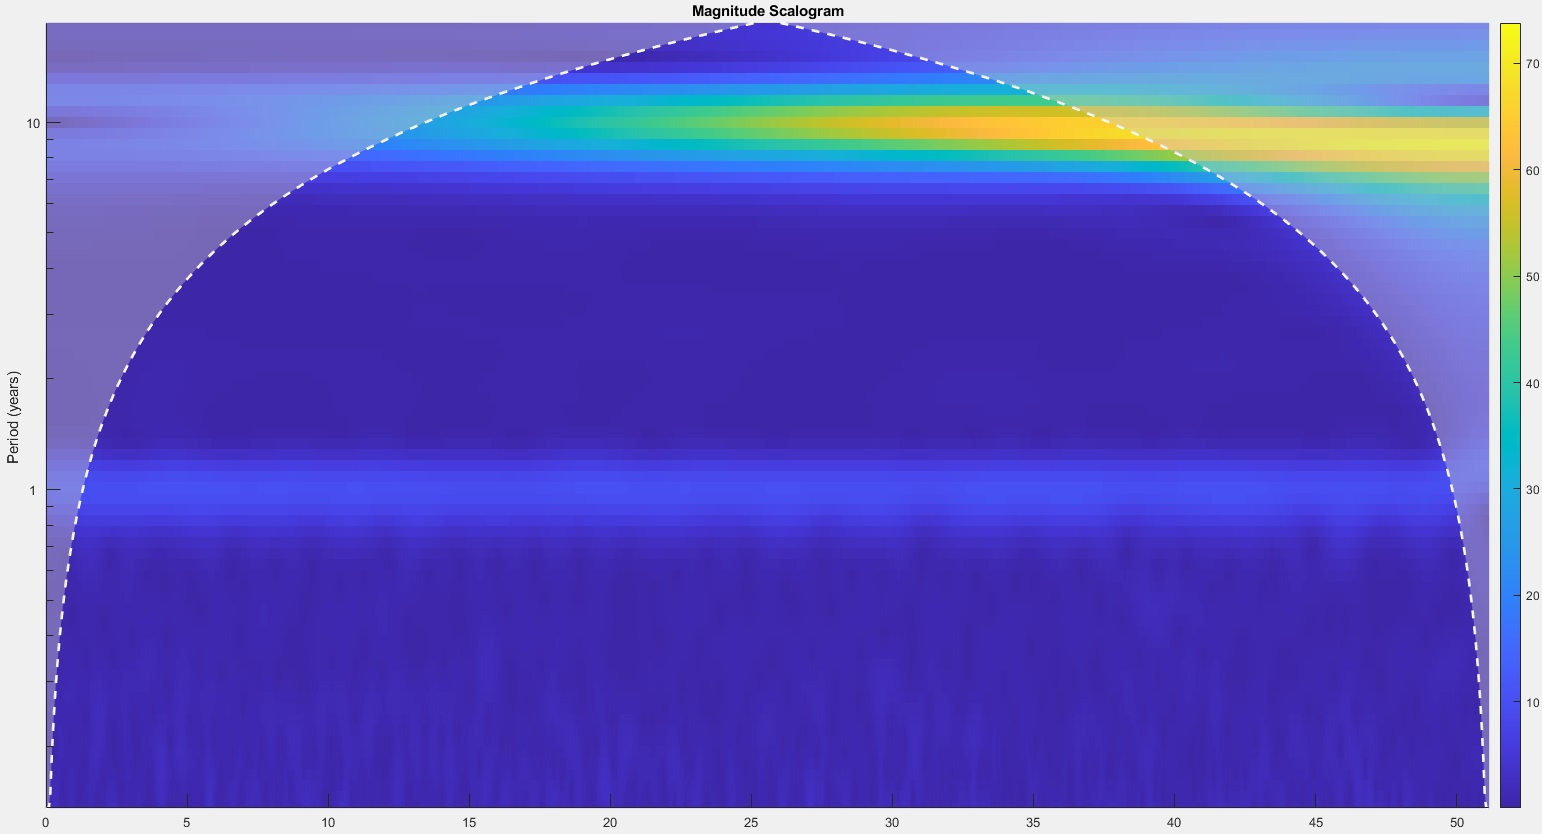
\includegraphics[width=1\linewidth]{inc/task1_vevlet1}}
	\caption{Вейвлет анализ сигнала из примера}
	\label{task1_vevlet1}
\end{figure}

\newpage
На рисунке \ref{task1_ssa1_not_grouped} представлен cингулярный спектральный анализ сигнала до группировки:

\begin{figure}[!h]
	\center{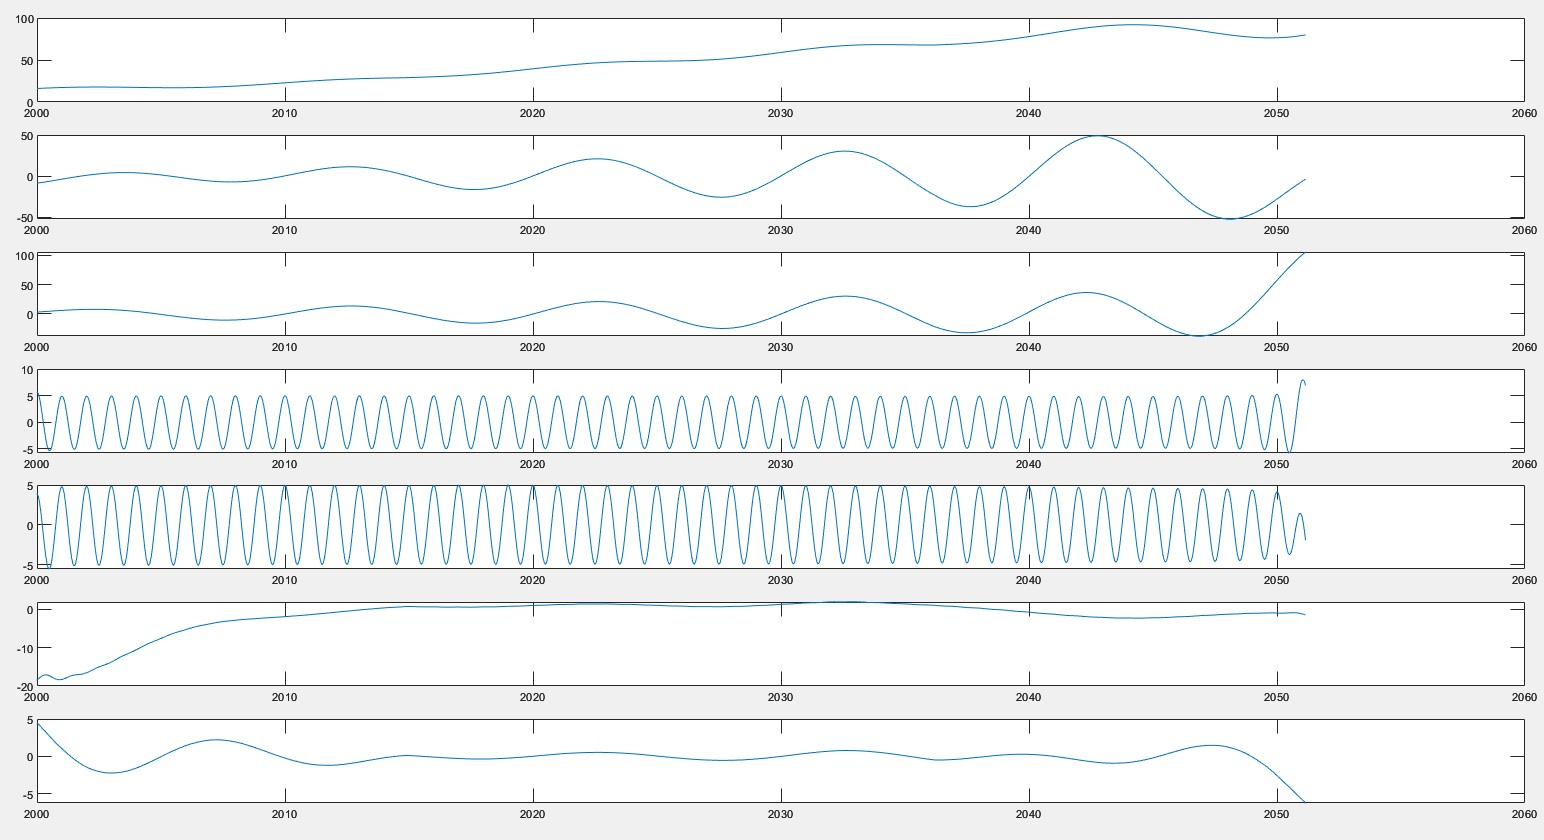
\includegraphics[width=1\linewidth]{inc/task1_ssa1_not_grouped}}
	\caption{Сингулярный спектральный анализ сигнала из примера до группировки}
	\label{task1_ssa1_not_grouped}
\end{figure}

На рисунке \ref{task1_ssa1} представлен cингулярный спектральный анализ сигнала после группировки:

\begin{figure}[!h]
	\center{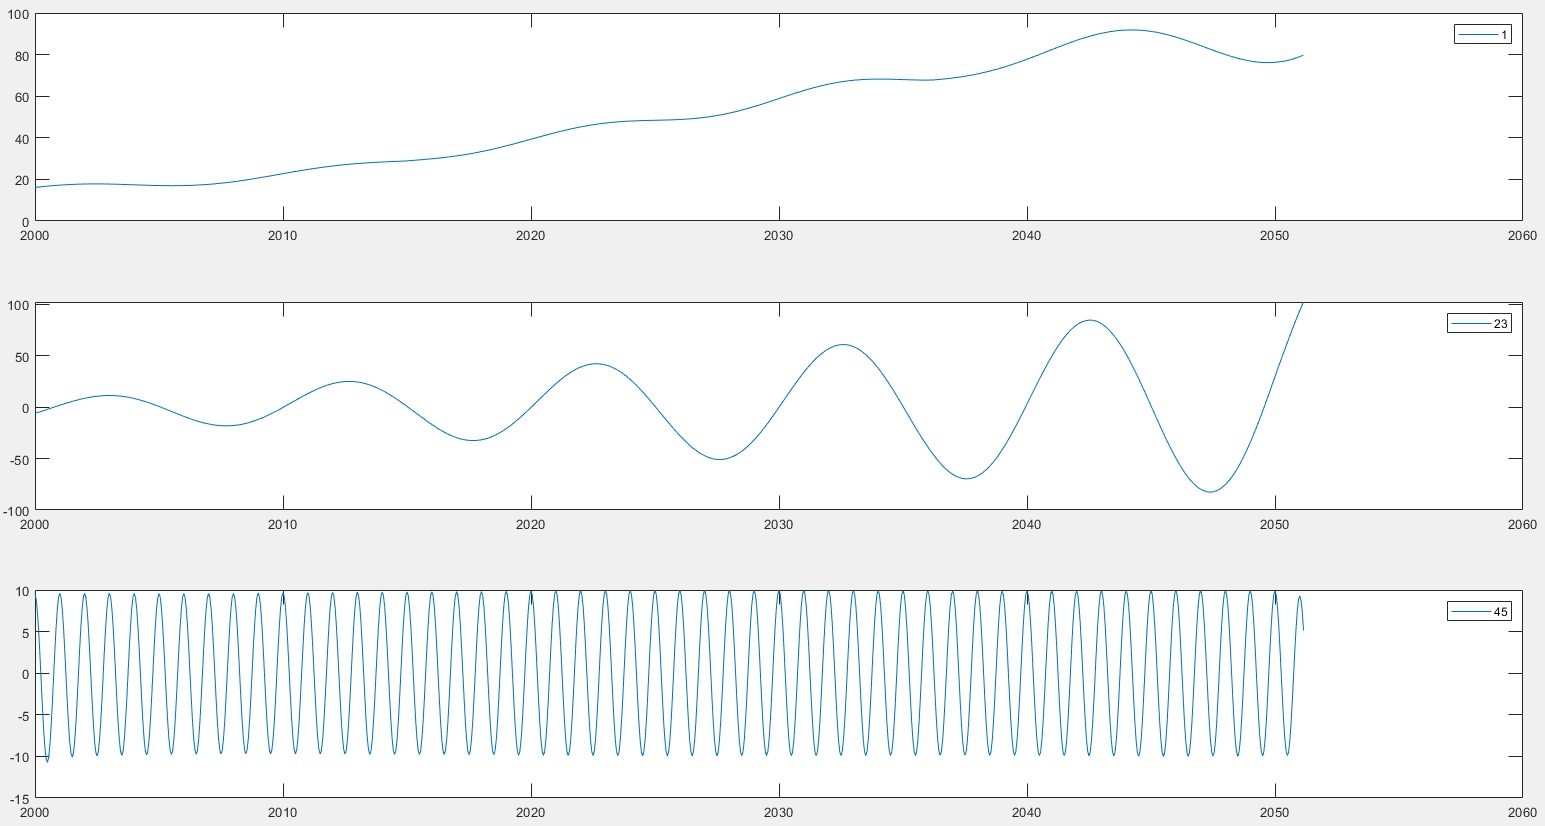
\includegraphics[width=1\linewidth]{inc/task1_ssa1}}
	\caption{Сингулярный спектральный анализ сигнала из примера после группировки}
	\label{task1_ssa1}
\end{figure}

На рисунке \ref{task1_ssa1}, на первом графике виден тренд, на втором низкочастотная гармоника, а на третьем высокочастотная.

\newpage
\noindent\textbf{Выводы:}

Фурье анализ хорошо выделяет частотные компоненты в данных, мы видим присутствие разных частот, но неизвестно в какие моменты эти частоты включаются. 

Вейвлет анализ показывает, что есть усиливающаяся низкочастотная гармоника, есть высокочастотная гармоника с не меняющейся амплитудой и есть какие то шумы.

Сингулярный спектральный анализ позволил определить как тренд, так и обе гармоники для сигнала из примера. ССА позволяет выявить как периодические, так и нелинейные тренды в данных, а также хорошо справляется с анализом временных рядов, содержащих различные временные масштабы.

%Вывод?

\newpage
На рисунках \ref{task1_garm2}-\ref{task3_ssa2} представлены аналогичные графики для сигнала из ЛР1.

Для начала, выведем сам сигнал из ЛР1 (рис. \ref{task1_garm2}):

\begin{figure}[!h]
	\center{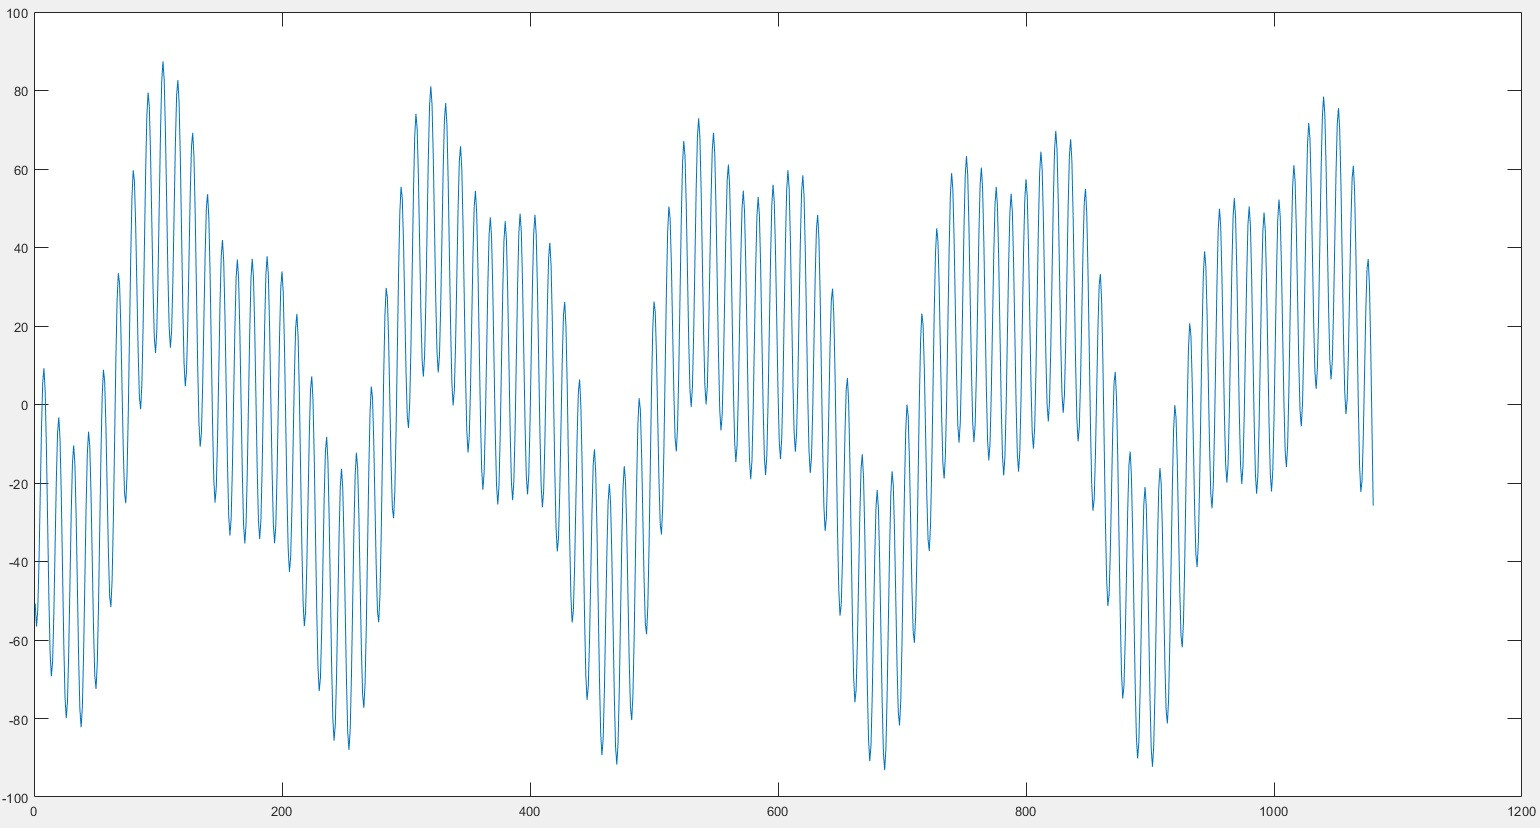
\includegraphics[width=0.9\linewidth]{inc/task1_garm2}}
	\caption{Сигнал из ЛР1}
	\label{task1_garm2}
\end{figure}

Затем составляющие сигнала и тренд (рис. \ref{task1_signal2}):

\begin{figure}[!h]
	\center{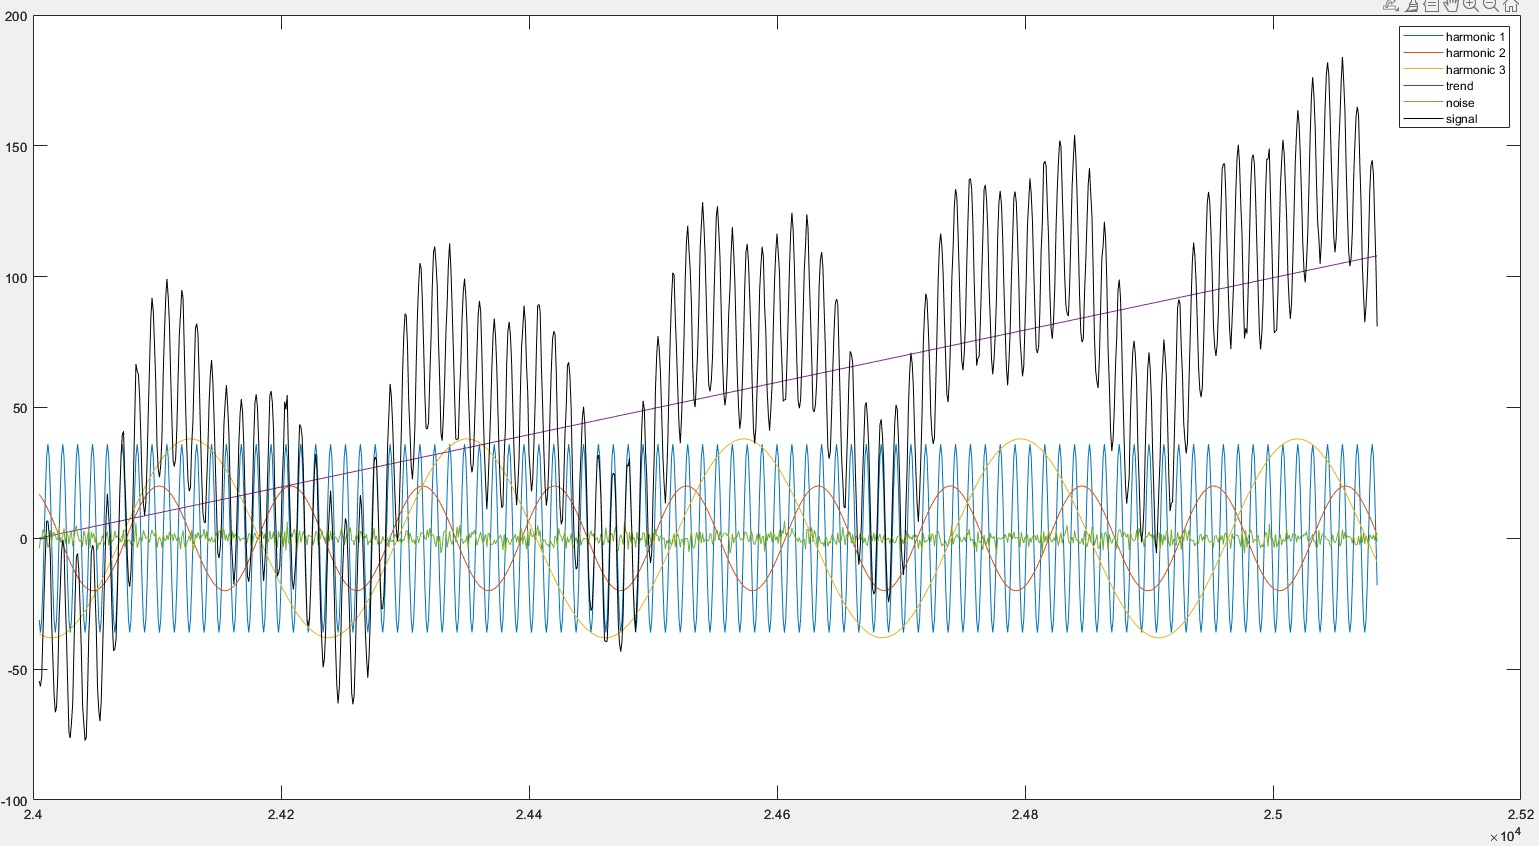
\includegraphics[width=1\linewidth]{inc/task1_signal2}}
	\caption{Сигнал из ЛР1 с шумом и его составляющие}
	\label{task1_signal2}
\end{figure}

\newpage
Применим Фурье и Вейвлет анализы (рис. \ref{task1_fft2}-\ref{task1_vevlet2})

\begin{figure}[!h]
	\center{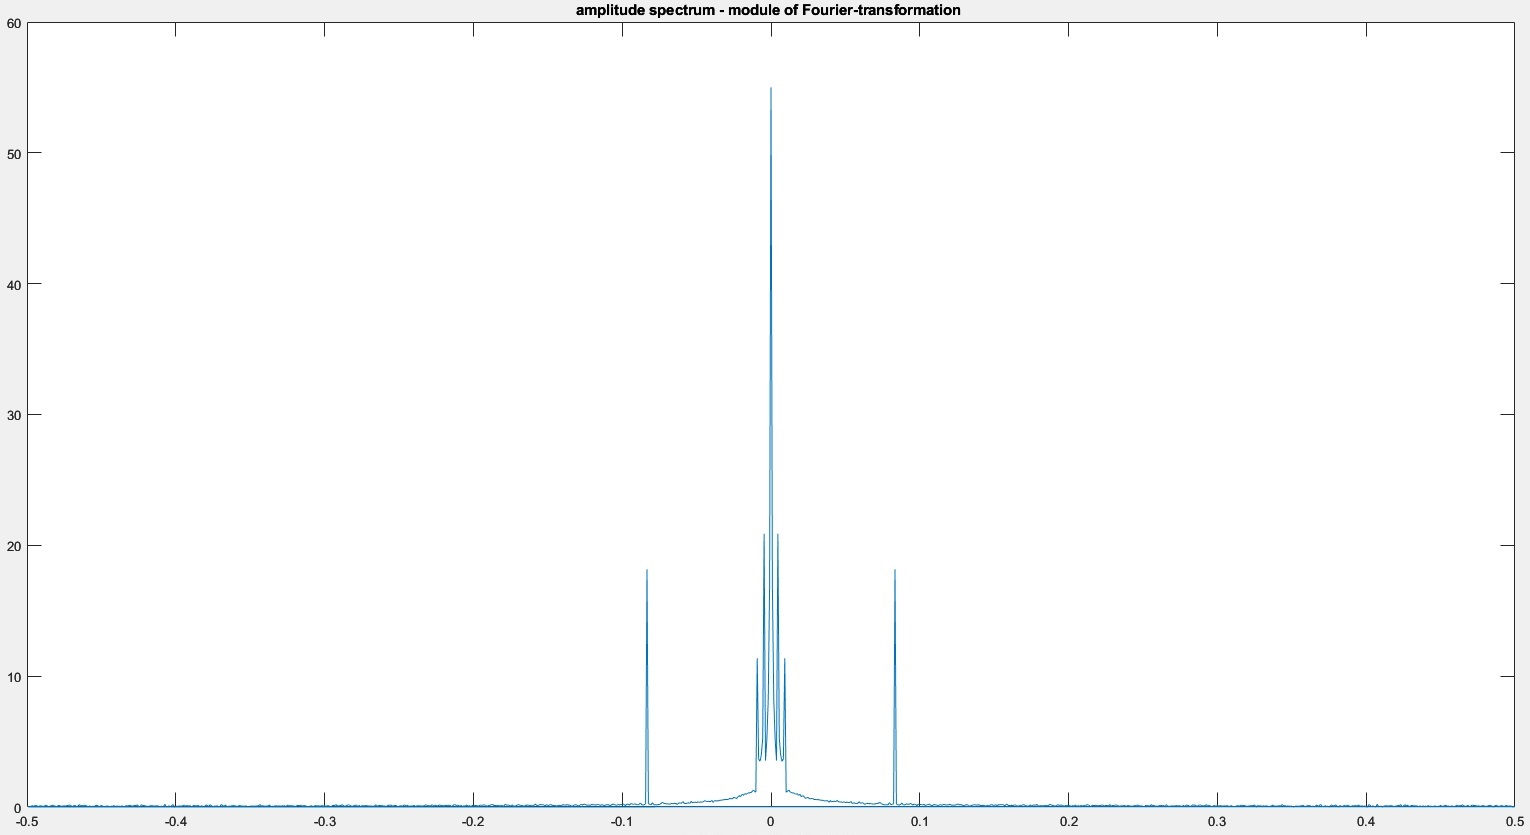
\includegraphics[width=1\linewidth]{inc/task1_fft2}}
	\caption{Фурье анализ сигнала из ЛР1}
	\label{task1_fft2}
\end{figure}

\begin{figure}[!h]
	\center{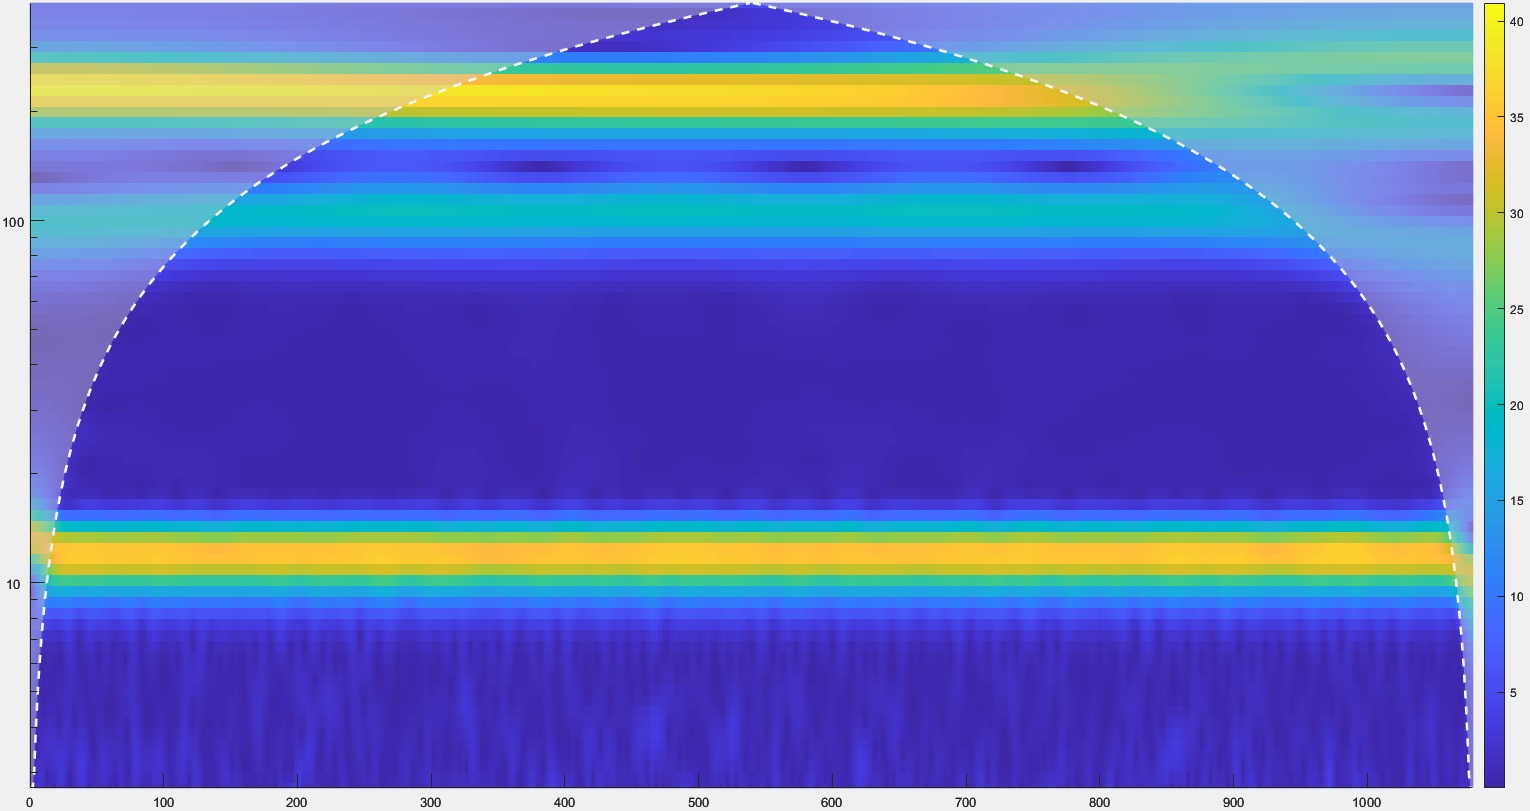
\includegraphics[width=1\linewidth]{inc/task1_vevlet2}}
	\caption{Вейвлет анализ сигнала из ЛР1}
	\label{task1_vevlet2}
\end{figure}

В результате обоих анализов, можно увидеть все три гармоники различной частоты и небольшой шум.

\newpage
Попробуем применить сингулярный спектральный анализ к этому сигналу с L=300 (рис. \ref{task3_ssa2_300})

\begin{figure}[!h]
	\center{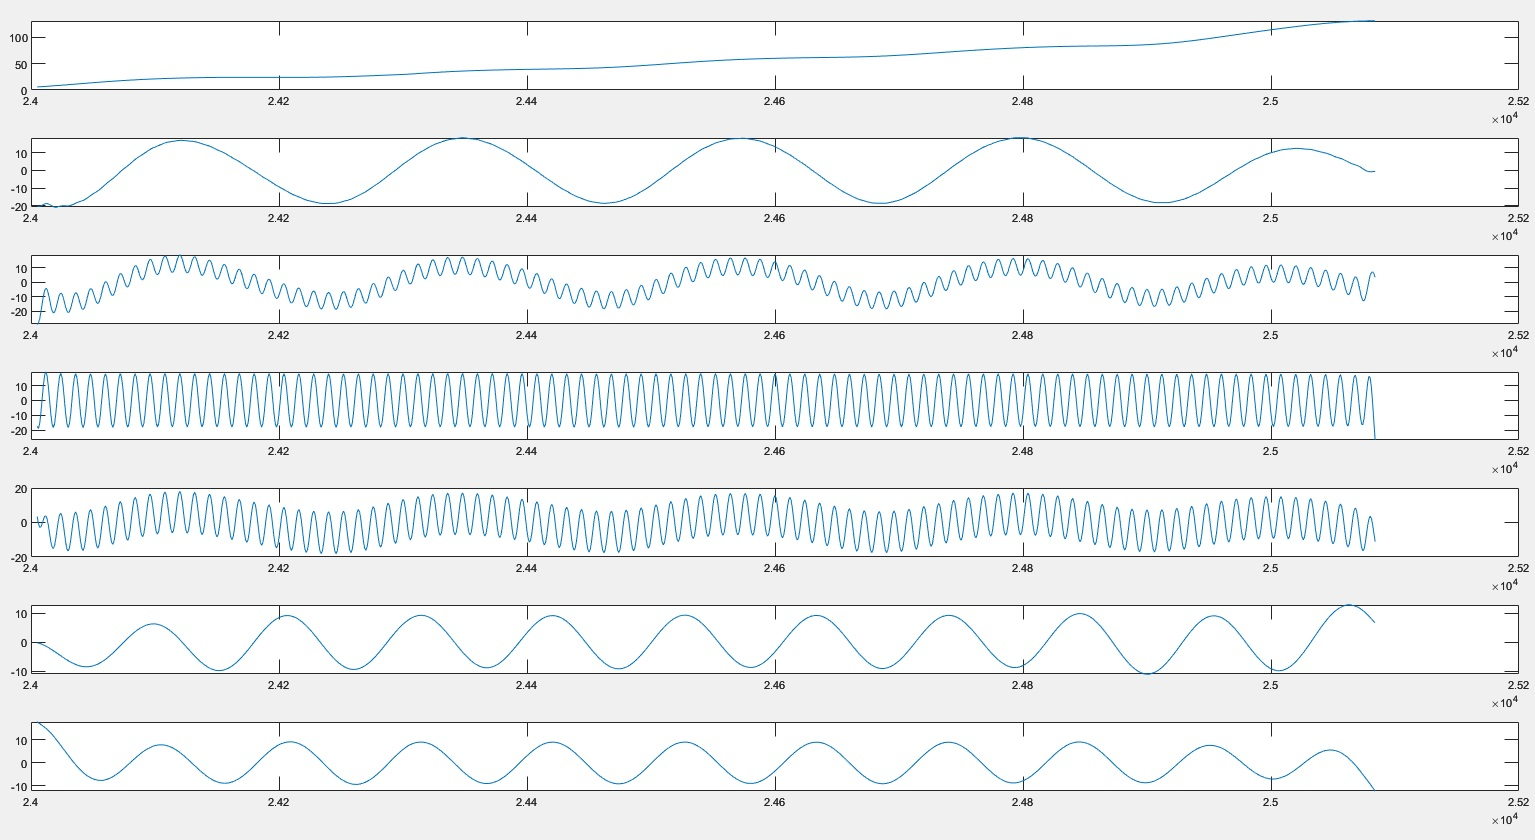
\includegraphics[width=1\linewidth]{inc/task3_ssa2_300}}
	\caption{Сингулярный спектральный анализ сигнала из ЛР1 при L=300}
	\label{task3_ssa2_300}
\end{figure}

По первому графику еще можно выделить тренд, а из второго низкочастотную гармонику, но уже на третьем графике видим смешанные частоты. Поэтому, попробуем поменять L на 350 (рис. \ref{task3_ssa2_350}):

\begin{figure}[!h]
	\center{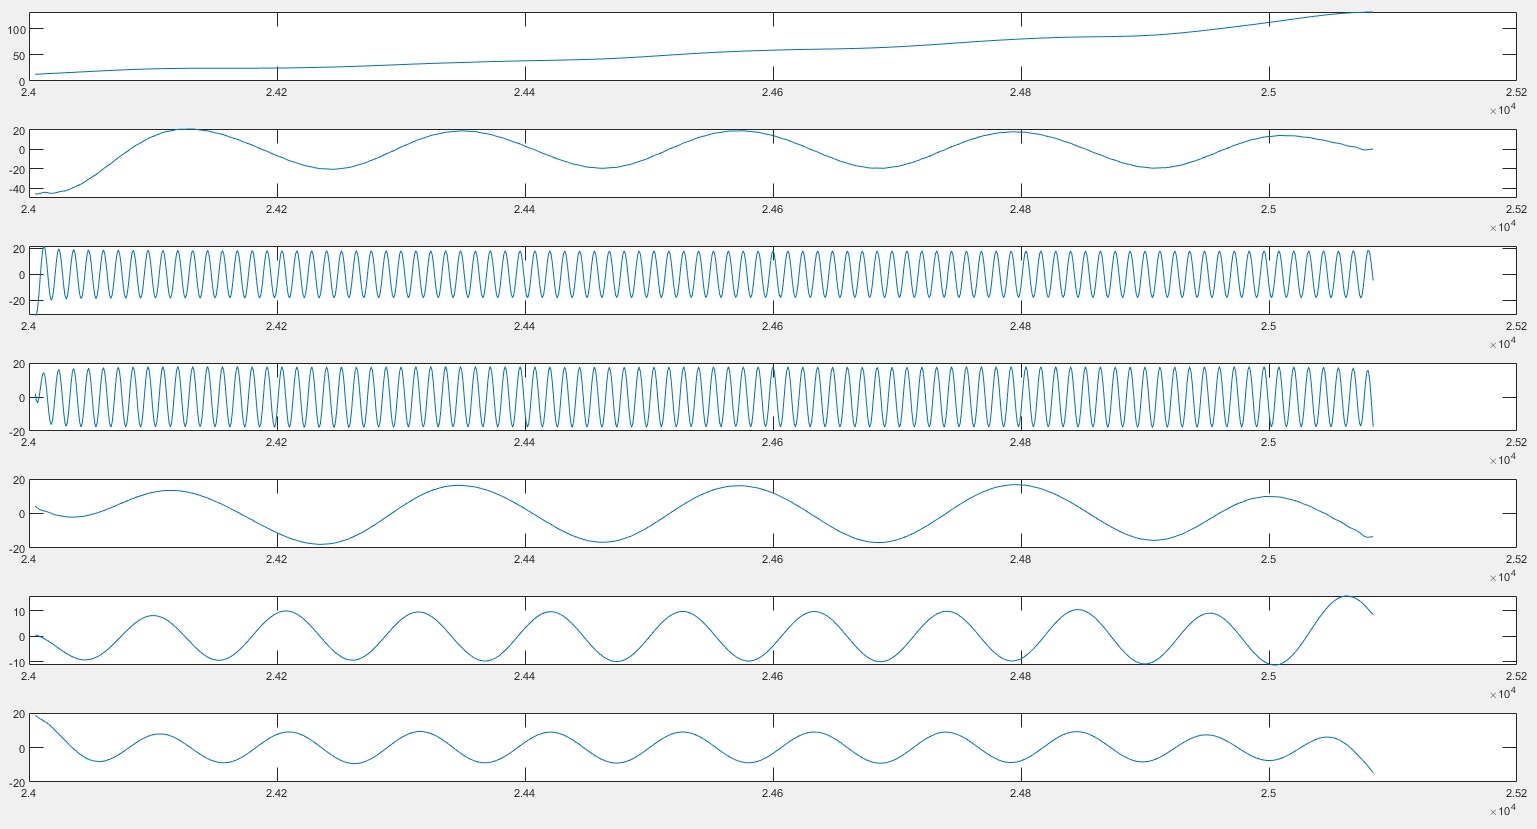
\includegraphics[width=1\linewidth]{inc/task3_ssa2_350}}
	\caption{Сингулярный спектральный анализ сигнала из ЛР1 при L=350}
	\label{task3_ssa2_350}
\end{figure}

\newpage
Теперь результат получился более приемлемым - видно что нужно сгруппировать графики: 2-ой с 5-ым (низкочастотная гармоника), 3-ий с 4-ым (высокочастотная гармоника) и 6-ой с 7-ым (среднечастотная гармоника). Так и сделаем:

\begin{figure}[!h]
	\center{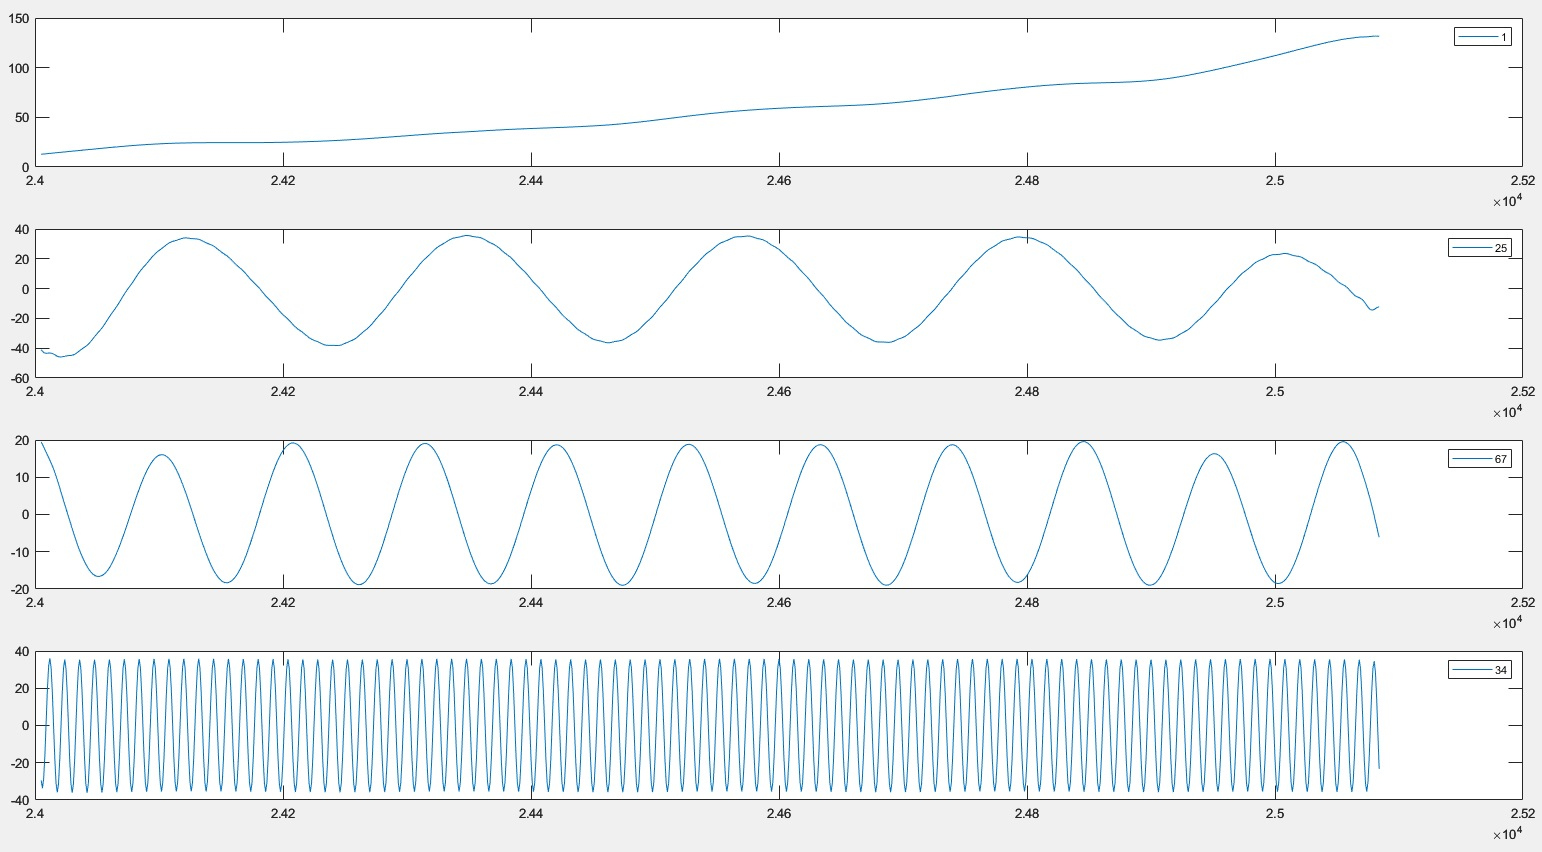
\includegraphics[width=1\linewidth]{inc/task3_ssa2}}
	\caption{Сингулярный спектральный анализ сигнала из ЛР1}
	\label{task3_ssa2}
\end{figure}

На рисунке \ref{task3_ssa2}, на первом графике виден тренд, на втором низкочастотная гармоника, на третьем среднечастотная, а на четвертом высокочастотная. Следовательно, можно сделать вывод, что с помощью сингулярного спектрального анализа также можно разделить сигнал на компоненты.

В зависимости от конкретной задачи и характера данных, каждый из методов (Фурье, Вейвлет и сингулярный спектральный анализы) может быть предпочтителен. Например, ССА может быть полезным для выделения нелинейных компонентов, вейвлет-анализ - для анализа локализованных структур, а Фурье-анализ - для выявления частотных характеристик периодических сигналов.

\end{document}